
\section{Présentation des cas }
    \label{section:detail_cas}

    Dans cette section, nous introduisons les sept structures étudiées dans le cadre de l'étude. Pour chacune, nous décrivons l'importance donnée aux quatre identités organisationnelles. L'importance relative de ces identités est représentée visuellement à l'aide d'un diagramme en radar. Nous détaillons ensuite les modalités de l'action environnementale dans ces organisations, ainsi que les facteurs qui motivent ou facilitent sa réalisation.

    \subsection{Air PACA}

        Air PACA est une association de surveillance de la qualité de l’air en PACA. Elle réalise cette mission avec un agrément de l’État auquel elle se substitue pour cette mission. Son rôle se décline en quatre volets : (1) la mesure et la surveillance de la qualité de l’air, (2) l’information du public et la sensibilisation aux enjeux, (3) l’accompagnement des acteurs privés et publics et (4) le développement des connaissances. Air PACA est en premier lieu caractérisée par sa \textbf{dimension collective}. En effet, elle est gouvernée par quatre collèges représentés de façon équitable : l’État, les collectivités territoriales, les industriels et les acteurs de la société civile. Son fonctionnement repose sur de nombreux partenariats et l’implication de nombreuses parties prenantes dans ses activités. \textbf{Les identités normative et fonctionnelle} sont intrinsèquement liées et principalement marquées par la mission d'intérêt général et environnemental (le cœur de métier de l’association étant directement lié à l’écologie). \textbf{L'identité utilitariste} fait apparaître un équilibre entre un fonctionnement entrepreneurial et une certaine logique de compétition, et des sources de financements prenant la forme de subventions ou de mécanismes fiscaux.

        \begin{figure}[h]
            \caption{Identités organisationnelles chez Air PACA}
            \label{figure:dimairpaca}
            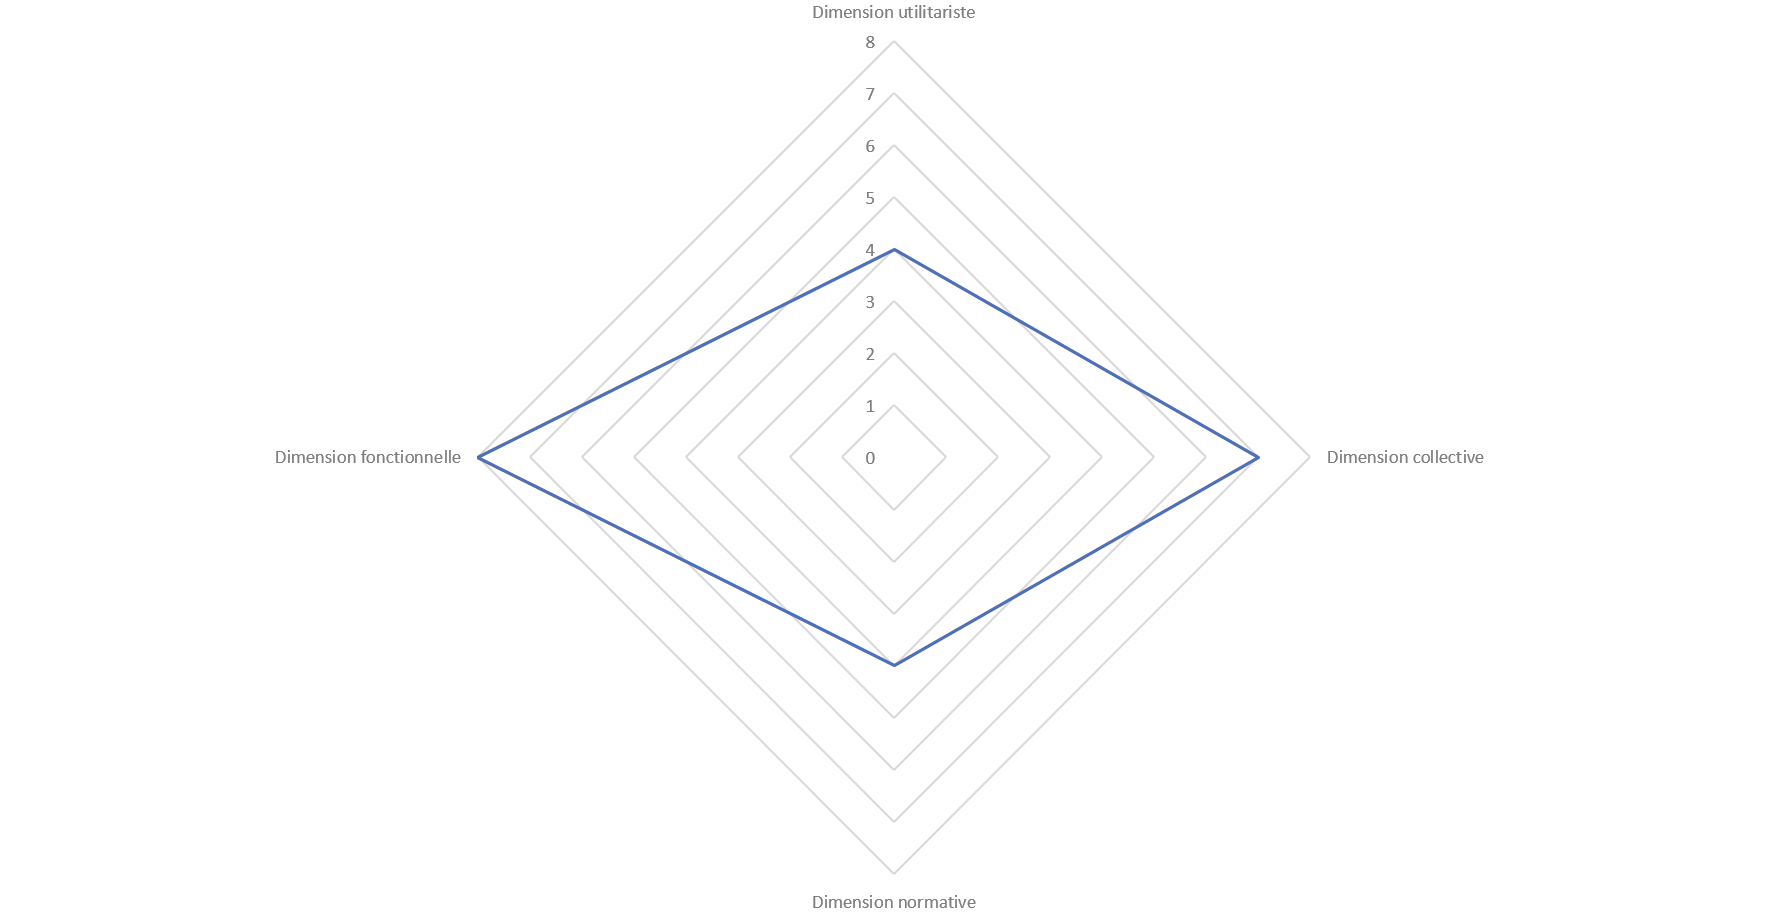
\includegraphics[width=\linewidth]{fig/radars/Air_PACA.png}
        \end{figure}

        L’association appréhende la qualité de l’air comme un enjeu à la fois de santé publique et de préservation de l’environnement. Le cœur de son activité est donc la réduction de la pollution de l’air. Dans ce cadre, l’association se montre très éco-innovante, notamment du point de vue de l’innovation technologique. Air PACA développe des nouveaux médias de communication des données, pour s’approcher d’une information en temps réelle de la qualité de l’air, destinée aussi bien à des particuliers qu’à des organismes privés ou publics. D’autres innovations technologiques portent sur des procédés individuels de mesure de la qualité de l’air, accessibles à tous.
        Ces innovations s’inscrivent pleinement dans une ambition de diffuser le plus largement l’information et de sensibiliser les publics aux enjeux de la qualité de l’air. Pour avoir un impact au niveau de la région, Air PACA porte des éco-innovations institutionnelles en agissant auprès des décideurs en amont des projets d’aménagement du territoire. Au niveau de son fonctionnement, l’association a mis en place l’application de la norme ISO 14001 afin de limiter l’impact de son action (consommation de papier ou d’énergie, gestion des déchets, transports). Ceci prend la forme d’éco-innovations sociales (changements de pratiques des salariés) et organisationnelles (maintien de plusieurs sites pour limiter les déplacements). \\


        La première motivation de l’association dans sa démarche d’éco-innovation est l’amélioration de la qualité de son service. Le secteur de la qualité de l’air connaît un regain d’intérêt mais accuse un retard par rapport à d’autres problématiques comme la question de l’eau. Par conséquent, il est indispensable de suivre les évolutions d’un secteur où beaucoup reste à faire.
        L’évolution des technologies, en particulier dans le champ de la communication, va dans le sens de la volonté de partager et diffuser l’information.
        L’association fait aussi face à une demande croissante des attentes sociétales. Cet intérêt en augmentation se traduit par une hausse importante des demandes d’intervention d’Air PACA, par exemple dans les écoles.
        L’éco-innovation s’inscrit également dans une logique de cohérence entre la mission et les pratiques : l’adoption de la norme ISO 14001 permet à l’association de montrer qu’elle s’applique à elle-même des pratiques responsables avant de les promouvoir aux autres.
        Enfin, le statut associatif pousse Air PACA à démontrer l’efficacité de son action pour maintenir sa légitimité. \\

        Si l’éco-innovation apparaît indispensable pour Air PACA, elle n’est, paradoxalement, pas au cœur de ses missions et donc pas dans son ADN. L’innovation fait donc face à des résistances au niveau de la gouvernance : certaines parties prenantes souhaitent recentrer l’activité sur la mission d’origine, quand d’autres reconnaissent l’intérêt d’éco-innover. Ceci est renforcé par la structure de la gouvernance, au sein de laquelle cohabitent des parties prenantes qui peuvent avoir des agendas très éloignés (un industriel du transport et une association de protection de l’environnement par exemple).
        Au niveau des changements internes, comme la réduction des consommations ou le tri, l’association fait face à des résistances humaines, certains salariés n’étant pas sensibilisés à ces questions et peu enclins à appliquer ces nouvelles pratiques. Des actions de sensibilisation sont donc nécessaires.
        Une barrière conséquente est la dépendance à des financements publics. Alors que la demande augmente, les moyens restent constants et conditionnés à des demandes régulières et chronophages. Le statut d’association est une limite à ces démarches, car il masque la spécificité d’Air PACA et sa mission d’intérêt général.
        Enfin, la dépendance à des partenaires peut également créer des blocages : la collecte des déchets est par exemple rendue difficile par le manque d’engagement de la ville en la matière. De manière plus importante, l’activité est encadrée par un agrément dont les termes peuvent changer rapidement et remettre en question toute l’action innovante de l’association.

    \subsection{AMS Environnement}

        \begin{figure}[h]
            \caption{Identités organisationnelles chez AMS Environnement}
            \label{figure:dimAMSenvir}
            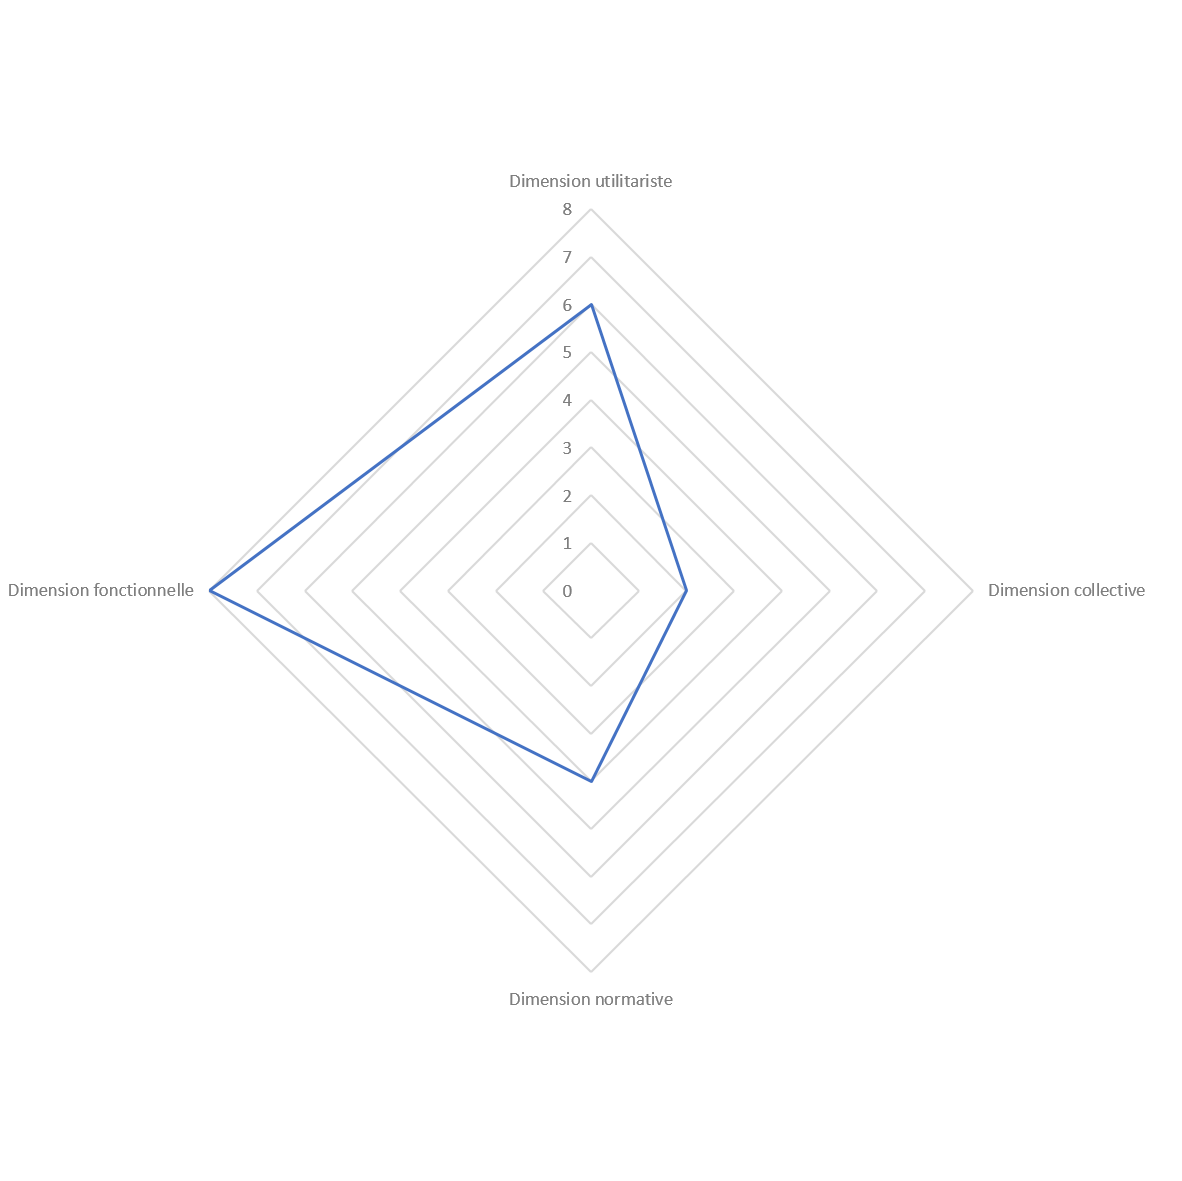
\includegraphics[width=\linewidth]{fig/radars/AMS.png}
        \end{figure}

        AMS Environnement est un chantier d’insertion sous format associatif basé à Aix-en-Provence. Sa mission est de salarier des personnes éloignées du travail pour les ramener vers le monde de l’entreprise. Le support de cette réinsertion est une activité d’entretien et de valorisation des espaces paysagers à destination des collectivités.

        Les différentes caractéristiques de l’ESS sont représentées de manière équilibrée. \textbf{L'identité normative} est marquée par un caractère militant, défendant une vision de l’insertion très centrée sur l’humain. L’association est portée par une volonté d’être acteur du développement durable. Sur \textbf{le plan utilitariste}, AMS revêt un caractère hybride. Le chantier d’insertion adopte un fonctionnement entrepreneurial mettant en avant sa dimension très professionnelle. Ceci est d’autant plus important que sa mission sociale est précisément de professionnaliser ses salariés en insertion. En revanche, 70 \% de ses financements proviennent de subventions. Les difficultés sociales de ses bénéficiaires, leur statut particulier ainsi que la \cit{plus-value humaine} éloignent également l’association d’une logique purement utilitariste. C'est donc avant tout l'\textbf{identité fonctionnelle}, c'est-à-dire la mission d'insertion, qui prime. La \textbf{dimension collective} est principalement marquée par des partenariats avec des acteurs publics lui permettant d’accéder à certains avantages (locaux mis à disposition par la mairie par exemple).  \\


        L’écologie n’est pas au cœur de la démarche de l’association et a été jusqu’ici laissée de côté ou prise en compte de manière marginale. Toutefois, l’organisation s’oriente maintenant vers des activités en lien avec l’écologie, en intégrant notamment les pratiques \cit{zéro-phyto}. En outre, l’association va prochainement acquérir un bâtiment à  basse consommation au Technopole de l’Arbois, justement afin de s’inscrire dans la dynamique environnementale portée à cet endroit.

        L’évolution vers des activités écologiques est principalement stratégique, utilitariste et répond à un enjeu de survie de l’organisation. La conviction de la direction est que leur secteur d’activité va s’orienter vers l’écologie, en particulier s’adressant à des acteurs publics soumis à des normes environnementales importantes dans la gestion de leurs espaces verts. Cette adaptation permet donc de répondre à une demande croissante et de se différencier, d’avoir une originalité par rapport à d’autres entreprises et chantiers d’insertion. La démarche environnementale initiée s’inscrit aussi en lien avec la mission sociale : la dimension écologique est jugée valorisante pour les bénéficiaires, quand l’insertion souffre justement d’une perception négative. L’enjeu des travaux réalisés est toujours expliqué aux employés en insertion afin de valoriser leur action.

        L’orientation écologique ne passe pas par de fortes innovations, mais plutôt par l’adoption de pratiques existantes. L’association ne se positionne pas comme un acteur fortement innovant ; elle fait évoluer son offre dans une direction qui lui semble pertinente stratégiquement. Or, si la demande est croissante, elle n’est pas encore suffisante pour justifier une orientation plus forte en ce sens. En outre, le financement d’activités plus écologiques est jugé encore insuffisant. L’innovation environnementale est également limitée par la grande priorité donnée au projet d’insertion. Le premier défi de l’association est d’avoir une activité réellement \cit{insérante}. C’est sur cet aspect que les efforts ont été principalement concentrés.


    \subsection{Groupe Arborescence}

        Arborescence est un groupe d’économie sociale organisé sous la forme d’une \scic dont sont membres cinq associations et coopératives œuvrant dans des activités autour de l’emploi, de la formation et de l’insertion. La \scic Arborescence assure les fonctions support (direction, administration…) de ces organisations afin de réaliser des économies d’échelle et de bénéficier d’un effet taille.

        \begin{figure}[h]
            \caption{Identités organisationnelles chez Arborescence}
            \label{figure:dimarborescence}
            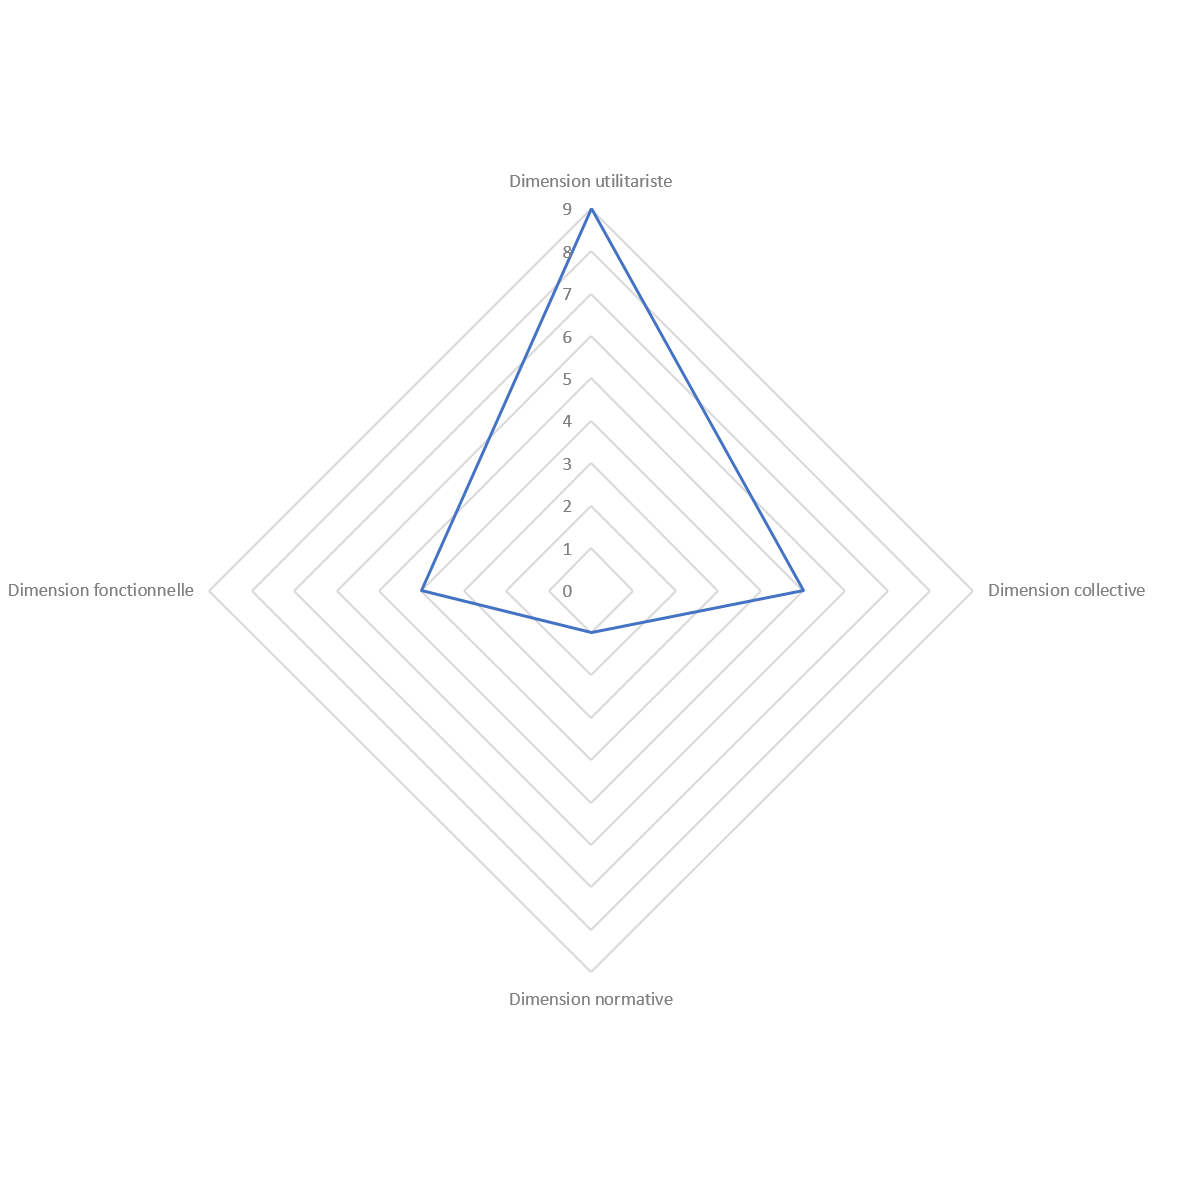
\includegraphics[width=\linewidth]{fig/radars/Arbo.png}
        \end{figure}

        La \scic applique un fonctionnement managérial classique similaire à une entreprise capitaliste (\textbf{identité utilitariste}). La dimension professionnelle est revendiquée et l’organisation formule ses objectifs en termes de résultats et de croissance. La structure coopérative est uniquement adoptée car son métier, l’insertion, est légalement prévu dans le cadre de l’ESS. A ce titre, l’entreprise reçoit des subventions publiques, mais valorise la possibilité d’aller chercher des marchés privés. La \scic se distingue uniquement du secteur classique par un accompagnement renforcé des salariés en insertion et une participation importante des salariés dans la décision. \textbf{L'identité collective} est en effet une caractéristique importante du groupe, la majorité des permanents ayant choisi de souscrire des parts et donc de participer à la gouvernance. \textbf{L'identité normative} est caractérisée par une appartenance historique au mouvement coopératif, sans que cet aspect soit central pour l’organisation et l'\textbf{identité fonctionnelle} repose sur l'activité des chantiers d'insertion. \\

        La stratégie d’Arborescence n’est pas orientée vers les questions environnementales, qui ne sont pas évoquées dans les organes de gouvernance. L’éco-innovation est guidée par les opportunités commerciales et de développement. Une entité du groupe intervient ainsi dans le nettoyage automobile avec des procédés écologiques. Cependant, celle-ci a été intégrée au groupe pour son activité d’insertion et non en raison de sa dimension écologique. Le secteur de l’insertion par les activités environnementales est perçu comme une niche, déjà très occupée par de nombreux acteurs en PACA, et offrant donc peu d’opportunités de développement. Il n’y a donc pas de volonté interne à se montrer éco-innovant.


    \subsection{Enfants et Loisirs}

        Enfants et Loisirs est une association loi 1901 qui détient une crèche et une micro-crèche à Saint-Cannat (13). La mission de l’association est la garde d’enfants la journée, associée à une mission éducative.

        \textbf{L'identité collective} est très importante dans l’association. Les membres sont les parents des enfants bénéficiaires des services de la crèche. Ils sont représentés par un conseil d’administration élu par l’assemblée générale. Bien que les salariés ne soient pas représentés dans la gouvernance, leur rôle est fortement mis en avant et les projets sont mis en œuvre de manière participative. \textbf{L'identité fonctionnelle}, à savoir l'accueil des enfants, la qualité du soin et de la pédagogie est centrale dans l'association. C'est à cette fin que sont mobilisées des valeurs sociales mais aussi environnementales initialement insufflées par la directrice (\textbf{identité normative}). \cit{L'identité utilitariste} est assez peu mise en avant. Les ressources sont majoritairement des subventions publiques mais une partie du service est payée par les membres (les parents). Soumise à des normes et agréée par le Conseil Départemental, l’association adopte toutefois une organisation professionnelle. \\

        \begin{figure}[h]
            \caption{Identités organisationnelles chez Enfants et Loisirs}
            \label{figure:dimenfantsetloisirs}
            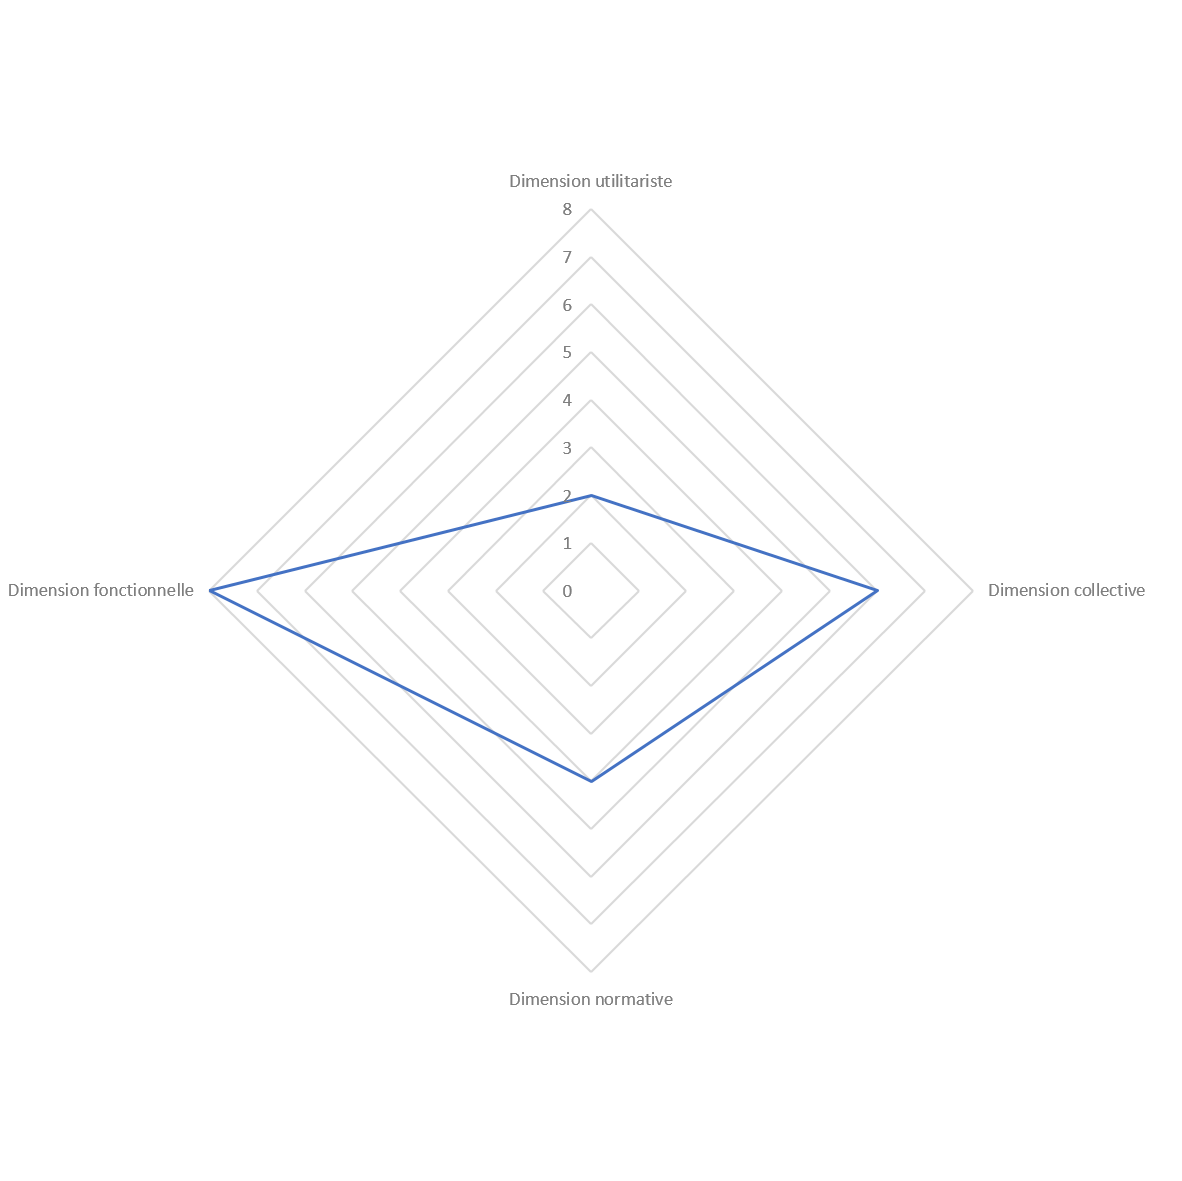
\includegraphics[width=\linewidth]{fig/radars/E&L.png}
        \end{figure}

        Depuis plusieurs années, à l’initiative de l’ancienne directrice de la crèche, l’association s’est engagée dans une démarche écologique valorisée par le label \cit{EcoloCrèche}. Accompagné par l’Atelier Méditerranéen de l’Environnement (AME), l’association a mis en place de nombreux changements dans son organisation et ses pratiques. On peut donner plusieurs exemples d’éco-innovations qui ont été portées. Des innovations technologiques tout d’abord, avec l’investissement dans des appareils de ménage à la vapeur afin de limiter l’utilisation de produits chimiques polluants et l’installation d’un composteur dans la cour. Des innovations organisationnelles également : l’adoption d’une alimentation biologique à la cantine, en s’approvisionnant en partie auprès de petits producteurs locaux ; la fabrication \cit{maison} des produits ménagers ou d’hygiène, mais aussi des peintures, pâtes à modeler, pâtes à sel… ; l’usage de produits de récupération pour fabriquer des jeux ; le recours à des partenaires s’inscrivant dans cette démarche pour proposer des animations aux enfants. De nouvelles activités ont été développées, comme l’organisation d’évènements visant à proposer des produits bio ou écologiques aux habitants du village ; la création d’un potager bio...

        La démarche d’éco-innovation n’a pas été motivée par des considérations marketing ou commerciales, qui ne sont pas un enjeu pour l’association, dans un contexte dépourvu de concurrence. Elle résulte d’une conviction que cette action constitue une responsabilité, voire un \cit{devoir}. L’association est notamment consciente de son rôle éducatif et de l’importance de l’apprentissage dès le plus jeune âge de comportements écologiques. Si l’initiative de cette démarche résultait d’une volonté personnelle, elle a obtenu une adhésion large qui a permis au projet d’aboutir. Cette adhésion s’est retrouvée aussi bien au niveau des membres de l’association (les parents, soucieux du bien être de leurs enfants et de préoccupations environnementales) qu’au niveau des équipes, conscientes de l’importance de la démarche. L’association a également obtenu le soutien de la commune, qui a validé le surcoût budgétaire entrainé par le projet. Le soutien des parties prenantes, mais aussi leur participation active a été un élément clé de la mise en place des éco-innovations.

         Si le projet écolocrèche a été un succès et a permis la mise en place de nombreuses éco-innovations, certains facteurs ont constitué des freins voir des blocages. Tout d’abord, le projet s’est confronté à des résistances humaines : bien que les équipes aient accueilli favorablement le projet, elles ont rapidement redouté une surcharge de travail. En effet, certaines innovations nécessitent un travail important en amont, comme la fabrication de la peinture ou des produits d’entretien. Un travail d’accompagnement et de formation a donc été nécessaire pour faciliter l’acceptation de nouvelles pratiques.  De ces inquiétudes, il a résulté un déséquilibre entre les ambitions de l’AG (les parents) et celles des équipes. Les parents étaient favorables à un projet très ambitieux, allant jusqu’à organiser des actions en dehors de la crèche (actions de sensibilisation auprès des habitants de la commune par exemple). Au contraire, les équipes préféraient un champ d’action plus restreint, centré sur l’enfant et sur les pratiques ayant un impact plus réduit sur la charge de travail. Enfin, la dépendance à certains partenaires réduit aussi les possibilités d’action de l’association, par exemple sur le choix d’une peinture écologique pour des locaux appartenant à la commune.

        Les innovations menées par Enfants et Loisirs vont au-delà de l’activité de la crèche et montrent une volonté de diffuser des pratiques respectueuses de l’environnement. Auprès des membres tout d’abord, c'est-à-dire des parents : des actions ont été menées pour sensibiliser les familles à ces enjeux et les encourager à reproduire des pratiques responsables chez eux. Même au-delà, l’association a souhaité sensibiliser les habitants de la commune, à travers des projets n’ayant pas de lien direct avec l’activité de crèche.

        Le projet Ecolocrèche a entrainé une augmentation de certains coûts (achat d’aliments bio, investissement dans des équipements d’entretien à la vapeur…). Toutefois, ceci ne semble pas avoir constitué un frein. Au contraire, les membres comme les partenaires ont accepté ce surcoût, étant conscients du réel bénéfice pour les enfants. La dimension associative joue ici un rôle essentiel : les décideurs sont motivés par la mission sociale (ici la garde de leurs enfants dans de bonnes conditions) plutôt que par une recherche de gain économique. Cependant, ce projet met en évidence une faiblesse liée à certains types d’éco-innovations, qui est le risque d’un retour en arrière. En effet, certaines innovations, notamment dans les pratiques, ne nécessitent pas seulement un investissement humain pour leur mise en place, mais aussi dans la durée. Par conséquent, le choix a parfois été fait de revenir aux anciennes pratiques. Il est intéressant de noter que les actions qui ont été maintenues sont celles qui touchaient directement à l’enfant, c'est-à-dire qui avaient un lien direct avec la mission sociale de l’association. Les actions plus ambitieuses, comme la sensibilisation au-delà du périmètre de la crèche, ont été abandonnées ou réduites.


    \subsection{Tour du Valat }

        La Tour du Valat est une fondation située au cœur de la Camargue, où elle a vocation à mener des programmes de recherche pour la préservation des zones humides (marais, lagunes, étangs, rizières…). La Tour du Valat est reconnue pour son expertise scientifique. En outre, la fondation dispose d’un domaine important en Camargue, sur lequel elle reproduit les activités traditionnelles camarguaises comme l’élevage, la chasse et la culture, qui sont utilisées comme terrain de recherche et d’innovation.

        La fondation est caractérisée en premier lieu par \textbf{une identité normative et une identité fonctionnelle} étroitement liées. Elles se matérialisent notamment par un fort attachement à des valeurs sociales mais surtout écologiques. L'organisation a été fondée sur la volonté d’un homme d’agir pour préserver la nature. Elle revêt un caractère militant, cherchant à faire évoluer les pratiques en vue de la sauvegarde des zones humides. La fondation a une volonté de réconcilier l’humain et la nature (et non de défendre la nature contre l’humain). \textbf{Le caractère collectif} est un volet essentiel pour la fondation et est en premier lieu matérialisé par des partenariats nombreux. Ceux-ci sont non seulement vecteurs de financements, mais permettent aussi à l’organisation d’exister et de peser institutionnellement. Les projets de la Tour du Valat font fréquemment intervenir des parties prenantes externes (experts, collectivités…) et donnent aussi un rôle important aux salariés. La fondation recherche un équilibre entre l’adoption d’un \textbf{fonctionnement managérial} et la préservation de sa mission environnementale et de ses valeurs. Le financement provient essentiellement des intérêts générés par le capital initial apporté par le fondateur, ainsi que d’une autre fondation qu’il a également créée. Le reste provient de partenariats et d’une activité marchande à la marge. \\


        \begin{figure}[h]
            \caption{Identités organisationnelles chez Tour du Valat}
            \label{figure:dimtourvalat}
            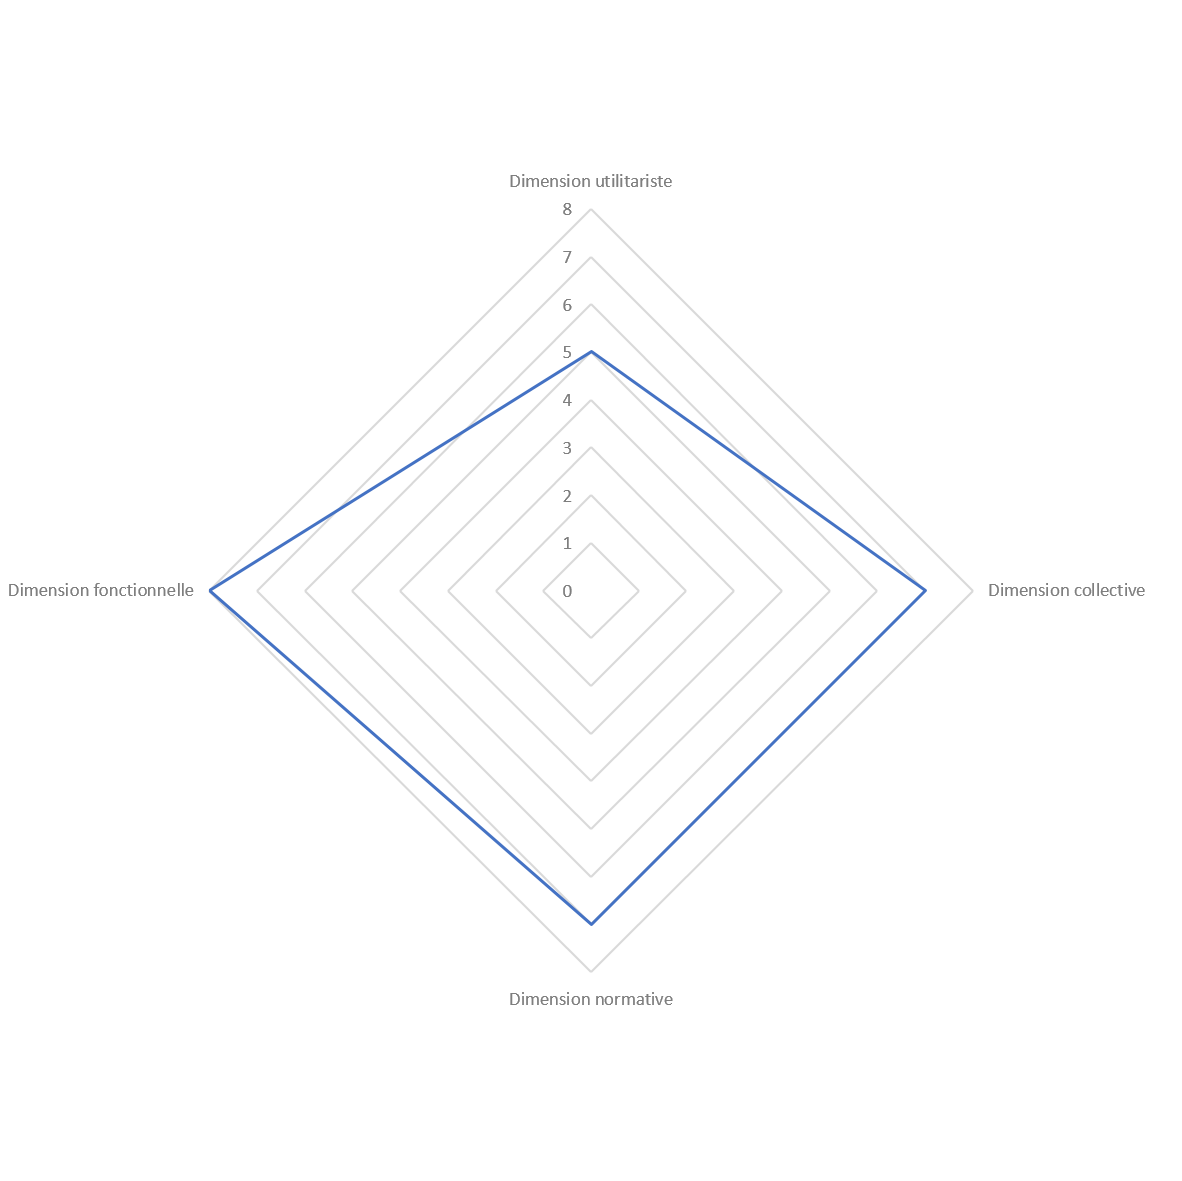
\includegraphics[width=\linewidth]{fig/radars/TdV.png}
        \end{figure}

        La Tour du Valat est par essence engagée dans l’action environnementale. Elle adopte un positionnement très éco-innovant, à différents niveaux. Elle met en place de nombreuses innovations, qu’elles soient technologiques (système de chauffage par chaudière à biomasse, isolation des bâtiments à l’aide de matériaux locaux comme la paille de riz…), sociales (mise en place d’un système de co-voiturage, mise en avant des transports en commun), organisationnelles (valorisation de la visio-conférence pour réduire les déplacements internationaux) ou institutionnelles (le programme de chasse a conduit à faire évoluer la législation en interdisant les balles en plomb pour réduire le saturnisme).

        Ces innovations répondent à plusieurs objectifs. D’une part, elles constituent une mise en cohérence avec les valeurs de l’entreprise et de ses salariés (déterminant interne). D’autre part, il s’agit d’appliquer à soi même ce qu’on préconise pour les autres et donc de légitimer son discours. En outre, ces éco-innovations répondent directement à la mission de l’organisation. Elles lui permettent de se constituer en vitrine, en modèle, pour montrer comment l’activité humaine est réconciliable avec la protection des écosystèmes. Les valeurs partagées au sein de l’organisation ont permis la mobilisation des équipes dans le cadre de ces innovations. Ceci a été un levier important pour la réussite de leur mise en place : certains projets ont ainsi été initiés et menés par les équipes.

        Paradoxalement, les comportements individuels sont aussi un obstacle important à l’éco-innovation, car ils sont parfois en contradiction avec les valeurs prônées. Une autre limite est le financement des éco-innovations, dont certaines ont un coût important. Le manque de moyens a conduit à un projet moins ambitieux et moins innovant pour l’isolation des bâtiments. Enfin, face à des projets très innovants, la fondation a parfois des difficultés à trouver des prestataires ayant l’expertise nécessaire à un coût accessible.

        Une dimension notable est la volonté de diffusion des innovations environnementales, qui résulte de la mission de l’organisation. Son rayonnement porte essentiellement sur le bassin méditerranéen et la fondation encourage l’application de techniques qu’elle a éprouvées dans d’autres écosystèmes comparables.


    \subsection{Provence Forêt}

        Provence Forêt est une coopérative agricole opérant dans la filière du bois et de la forêt. Elle rassemble des propriétaires forestiers dans une perspective de mutualisation des moyens, les parcelles étant généralement trop petites pour être gérées individuellement de façon rentable. Elle assure la valorisation (achat-vente) du bois de ses membres et propose également plusieurs services en lien avec la gestion durable de la forêt. Elle a donc deux catégories de clients : les acheteurs de bois (scieries, papeteries…) et ses membres à qui elle propose des services d’accompagnement.

        \begin{figure}[h]
            \caption{Dimensions de l'ESS chez Provence Forêt}
            \label{figure:dimprovenceforet}
            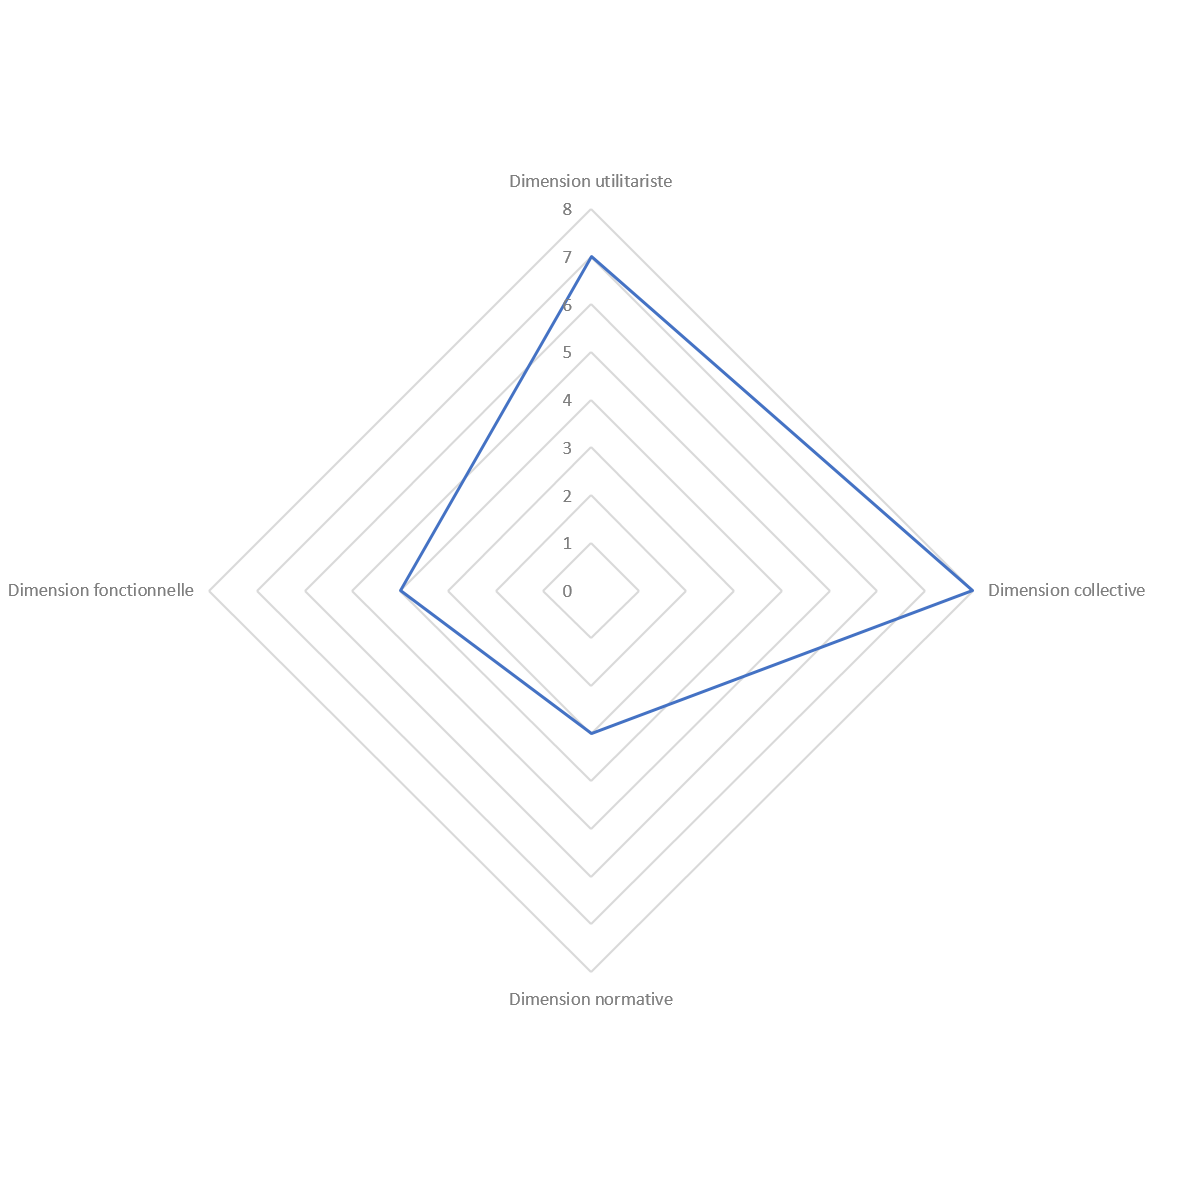
\includegraphics[width=\linewidth]{fig/radars/PF.png}
        \end{figure}
        Assez naturellement pour une coopérative, la dimension la plus marquée est \textbf{l’aspect collectif}. Celui-ci résulte d’abord de la participation des membres, à savoir des propriétaires forestiers, dans la gouvernance. En outre, celle-ci est également ouverte aux salariés (associés non coopérateurs). Mais la coopérative travaille aussi avec de nombreux partenaires. En particulier, l’obtention de plusieurs certifications s’est faite en collaboration avec un groupe de coopératives forestières de différentes régions. L'\textbf{identité utilitariste} est marquée par un fonctionnement entrepreneurial aussi bien dans les ressources financières (seuls 5 \% du chiffre d’affaires provient de subventions) que par un fonctionnement professionnel et très formalisé, organisé selon les normes ISO et PEFC. La structure n'est pas dotée d'une mission sociale ou environnementale, mais plutôt économique (\textbf{identité fonctionnelle}). Le rôle de l'organisation est la fourniture d'un service aux propriétaires forestiers et la valorisation de la filière en région \paca.
        \textbf{L'identité normative} est assez peu représentée, malgré une reconnaissance de la spécificité coopérative et des valeurs sociales et écologiques, existantes mais peu mises en avant. La coopérative insiste toutefois sur son ambition : proposer une gestion durable des forêts. L'appartenance à l'\ess tient surtout dans son format coopératif qui valorise la participation des membres et donne la priorité à la qualité du service et des conditions de travail avant la recherche de croissance du chiffre d'affaires.\\



        La coopérative est confrontée à un contexte environnemental complexe. A la réglementation importante de la filière s’ajoute la superposition des zones environnementales qui sont très nombreuses en \paca et dont il faut tenir compte.  Enfin, les effets du réchauffement climatique, notamment les phénomènes de sécheresse, se ressentent sur les arbres et donc sur l’activité.

        La démarche environnementale de la coopérative se matérialise surtout par l’obtention des certifications ISO14001 et PEFC qui valident une prise en compte de l’environnement et une gestion durable des forêts (éco-innovations de type organisationnel). La plupart des actions menées en faveur de l’environnement s’inscrivent dans le cadre de ces certifications. Celles-ci ont eu principalement des impacts organisationnels, à travers la formalisation de l’activité dans des procédures. Des réorganisations ont été faites pour limiter l’impact sur l’environnement, comme l’optimisation des déplacements en voiture des techniciens pour réduire le kilométrage.

        Les certifications environnementales répondent d’abord à des objectifs financiers et des objectifs d’image. La certification PEFC résulte d’une demande des clients qui ont besoin de se fournir en bois ayant ce label et qu’ils sont prêts à payer plus cher. L’obtention de cette certification en groupe nécessite préalablement une certification ISO. L’ISO 14001 s’est révélée pertinente au vu de l’impact de l’activité sur l’environnement. La démarche répond aussi à un enjeu d’image, la filière bois souffrant d’une mauvaise réputation auprès du grand public. La contestation peut se manifester de manière violente et questionner la légitimité même de la filière, et donc de la coopérative. L’application des normes ISO 14001 et PEFC a aussi été motivée par les bénéfices indirects sur l’activité. Le respect des procédures a conduit à réduire de façon importante le nombre d’accidents, dans un métier réputé dangereux. Les procédures mises en place permettent aussi de garantir le bon respect des réglementations, auxquelles il est facile de déroger involontairement lorsque l’activité n’est pas formalisée. L’obtention des certifications a été considérablement facilitée par la participation au Groupe Coopération Forestière qui avait déjà entamé le processus avant d’être rejoint par Provence Forêt. Les partages d’expériences ont constitué un atout considérable pour faciliter la réorganisation. Enfin, si les motivations sont principalement pragmatiques, l’action environnementale répond aussi à des valeurs environnementales partagée dans la coopérative, notamment au niveau des organes de gouvernance, et la conviction que l’industrie forestière ne doit pas être destructrice de l’environnement.

        La mise en place des certifications a été confrontée initialement à des résistances humaines, venant des salariés inquiets d’une complexification inutile du travail, à travers des procédures et des tâches administratives. D’autres projets d’éco-innovation sont envisagés par Provence Forêt, mais le manque de temps disponible des salariés et de ressources financières ne le permet pas. Ces projets portent notamment sur la recherche de nouvelles façons de planter ou de couper les arbres, ainsi que de nouvelles espèces plus adaptées à l’évolution du climat. Les partenariats viennent parfois compenser ses faiblesses, d’autres coopératives plus anciennes et plus solides financièrement étant fortement engagées dans ces actions de R\&D.

    \subsection{Bzzz}

        Bzzz est une association basée dans le Var, organisée sous la forme d’une AMAP, qui produit du miel et des produits dérivés de l’apiculture. Elle a aussi pour mission d’avoir une action de promotion de \cit{l’apiculture alternative}, de diffusion des connaissances et de militantisme auprès des pouvoirs publics.

        \begin{figure}[h]
            \caption{Identités organisationnelles chez Bzzz}
            \label{figure:dimbzzz}
            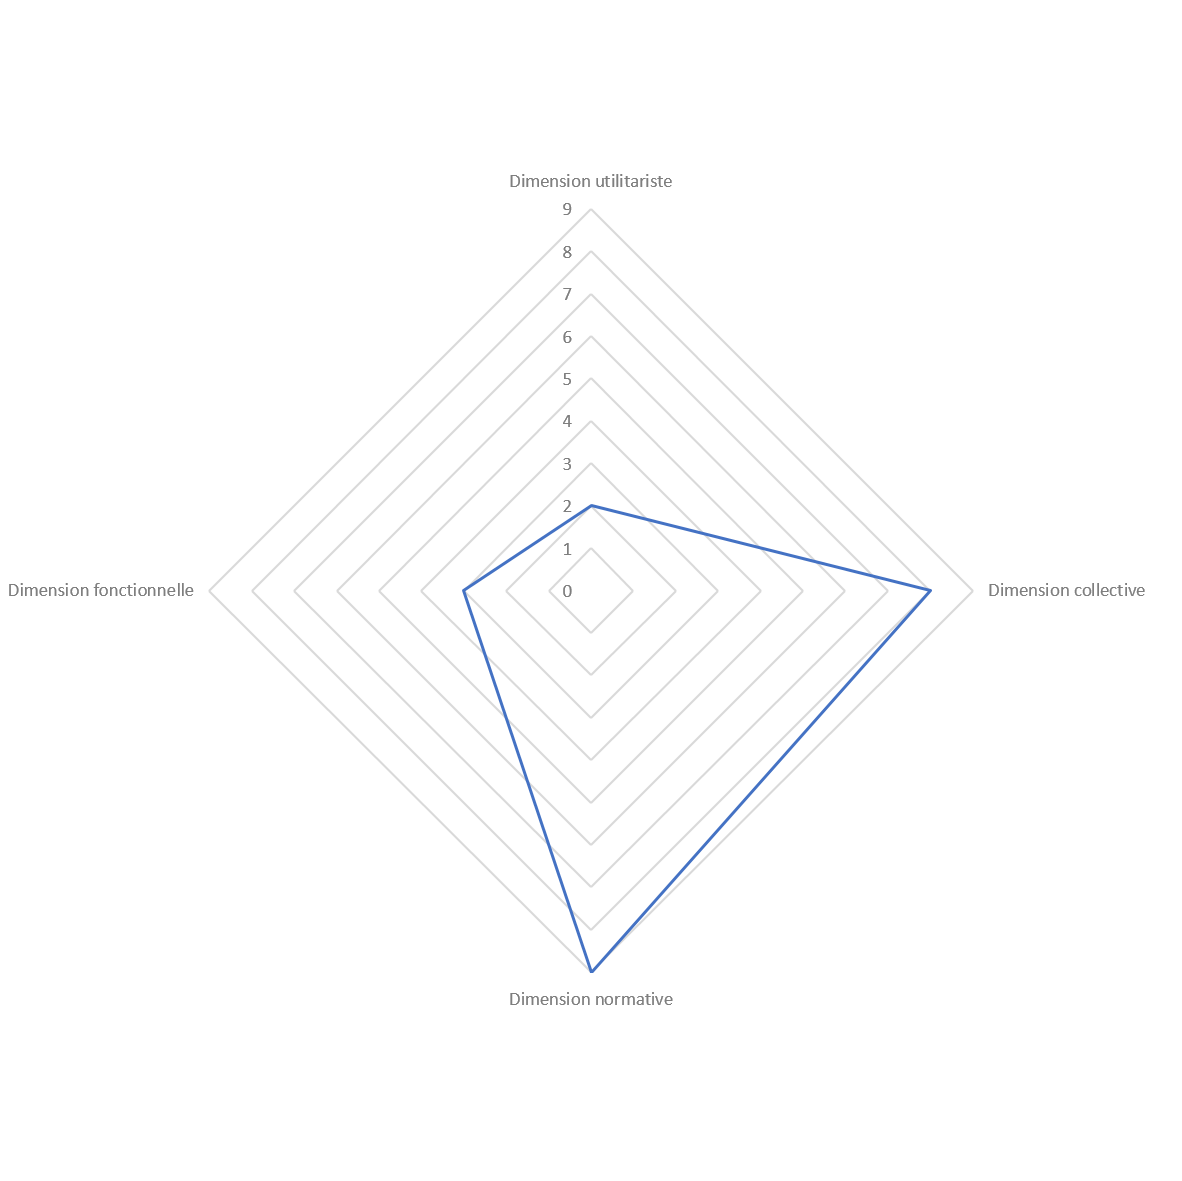
\includegraphics[width=\linewidth]{fig/radars/Bzzz.png}
        \end{figure}

        Bzzz est caractérisée d’abord par une forte \textbf{identité normative et collective}. Sur le plan collectif, l’association attache une importance majeure aux partenariats en particulier dans le milieu associatif, mais aussi auprès des acteurs publics. Ces partenariats permettent d’accéder à des compétences spécifiques, de peser collectivement sur les pouvoirs publics, de diffuser leur modèle et leurs idées ou d’accéder à des financements. L’association s’attache à faire participer à ses actions non seulement les salariés mais aussi des parties prenantes externes. De nombreuses actions sont portées collaborativement avec d’autres organisations. Les partenariats sont également motivés par une vision de l’économie qui ne repose pas sur le principe de concurrence, mais plutôt de collaboration et de co-construction. Ils s’inscrivent donc en lien avec une forte dimension militante de l’association, motivée par des valeurs écologiques et sociales très fortement ancrées. Bzzz porte la vision d’une apiculture alternative, mais aussi d’une autre façon d’envisager l’économie, refusant d’être uniquement guidée par des logiques de performance et de croissance. Ces valeurs sociales, écologistes et collaboratives constituent une finalité pour l'association (\textbf{identité fonctionnelle}), davantage que la production et la vente de miel et produits dérivés. Sur \textbf{le plan utilitariste},  Bzzz cherche un équilibre entre l’intégration de ses valeurs à son mode de fonctionnement et les contraintes économiques auxquelles elle fait face. Ainsi l’association fonctionne avec des salariés, valorise des sources de financement privées et fait preuve de professionnalisme dans la fabrication des produits vendus à ses membres, afin de s’assurer de leur bonne qualité. En revanche, elle revendique un management différent, plus humaniste, et rejette les logiques de performance ou la fixation d’objectifs trop contraignants qui pourraient l’éloigner de sa philosophie. L’association survit en outre grâce à des financements publics, toujours indispensables à ce jour. \\


        L’écologie est au cœur de la mission de l’association et s’inscrit pleinement dans sa démarche militante. Toute son approche de l’apiculture se veut alternative et innovante, et s’inscrit dans l’idée d’un respect de l’humain et de la nature. Par conséquent, de nombreux exemples d’éco-innovations sont observés. La logique de collecte du miel, qui vise à ne pas \cit{voler} aux abeilles ce qui leur appartient, mais à simplement extraire le surplus, se distingue de l’apiculture classique. Bzzz s’appuie sur un cheptel très restreint afin de privilégier la qualité. Des innovations technologiques ont également vu le jour, comme la fabrication d’une miellerie-savonnerie mobile à des fins de production mais aussi à visée pédagogique. Sur le plan institutionnel, l’association a contribué a faire évoluer des réglementations sur l’installation de ruches à Marseille et à réhabiliter une miellerie non utilisée par la ville. Bzzz porte actuellement un projet de création d’une mare et de plantation d’arbres afin de reconstituer un milieu favorisant les pollinisateurs.

        L’éco-innovation est clairement impulsée par l’engagement très fort de l’équipe de Bzzz et par la conviction de la nécessité et de l’urgence d’agir en faveur de l’environnement. Elle est l’essence même de l’association. L’innovation est également indispensable à la survie de l’association qui fait face à un contexte environnemental très difficile. Bien que l’association dispose de peu de ressources financières, des projets parviennent à être portés grâce à des partenariats. La \cit{Bzzz-mobile}, exemple d’éco-innovation technologique, a ainsi été développée à l’aide de plusieurs associations partenaires qui ont apporté les compétences nécessaires ainsi qu’un soutien financier. Les valeurs partagées avec ces partenaires sont un moteur de l’éco-innovation chez Bzzz. Enfin, la spécificité associative de Bzzz lui permet d’accéder à des financements particuliers et d’avoir recours à du crowdfunding en vue de projets donnés. Le projet de rucher actuel s‘inscrit dans le cadre du financement public \cit{Mon Projet Pour la Planète}, qui prend la forme d’une présélection administrative suivie d’un vote citoyen.

        Le modèle de Bzzz est principalement mis en difficulté par un contexte environnemental très difficile qui menace la survie des abeilles. Les sécheresses répétées, l’usage excessif de pesticides dans les exploitations agricoles alentour et la prolifération de prédateurs comme le frelon ont conduit à des récoltes de miel très faibles, voir nulles. L’association est donc confrontée à un enjeu de survie à très court terme et envisage de faire évoluer son modèle. La dimension financière est un enjeu particulièrement important. La difficulté d’obtenir des financements, aussi bien en raison de la charge de travail que des délais d’obtention des fonds, complexifie davantage les choses.

    \transition
    
    Les composants des identités organisationnelles des cas étudiés sont synthétisés dans le tableau \ref{table:synthesedimess}.

    \begin{footnotesize}
     \begin{landscape}
     \begin{longtable}{
         |>{\setlength{\baselineskip}{0.75\baselineskip}}K{0.1\linewidth}
         |>{\setlength{\baselineskip}{0.75\baselineskip}}K{0.2\linewidth}
         |>{\setlength{\baselineskip}{0.75\baselineskip}}K{0.2\linewidth}
         |>{\setlength{\baselineskip}{0.75\baselineskip}}K{0.2\linewidth}
         |>{\setlength{\baselineskip}{0.75\baselineskip}}K{0.2\linewidth}|}

         \caption{Synthèse des cas sous l'angle de l'identité organisationnelle}
         \label{table:synthesedimess} \\ \hline
          \textbf{Source}	& \textbf{Identité utilitariste}	& \textbf{Identité normative}	& \textbf{Identité collective} & \textbf{Identité fonctionnelle}\\ \hline

          \endfirsthead         \hline
          \textbf{Source}	& \textbf{Identité utilitariste}	& \textbf{Identité normative}	& \textbf{Identité collective} & \textbf{Identité fonctionnelle}\\ \hline
          \endhead

        Air PACA
        & Organisation interne classique, formalisation de l'activité à travers des certifications.
        & Mise en avant de l'intérêt général en lien avec l'action environnementale.
        & Gouvernance collégiale (4 collèges : État, collectivités, industriels, associations de protection de l'environnement).
        & Accent mis sur la notion d'intérêt général de la mission de l'association : surveillance et information sur la qualité de l'air.
        \\ \hline

        AMS Environnement
        & Activités menées de façon similaire à une entreprise classique. Recherche de financements de marché.
        & L'humain est mis au centre des missions de l'association, avec une approche personnalisée.
        & La gouvernance intègre des acteurs externes qui apportent des compétences. Cette dimension n'est toutefois pas fortement mise en avant.
        & Les équipes sont prioritairement concentrées sur la mission d'insertion : l'objectif de l'association est d'être \cit{véritablement insérante}.
        \\ \hline

        Groupe Arborescence
        & Fonctionnement similaire  à une entreprise de marché : le statut de coopérative est choisi uniquement pour mener l'activité d'insertion.
        & Le lien avec l'ESS tient dans l'importance donnée au principe de démocratie.
        & Participation de la quasi-totalité des salariés à la gouvernance de l'entreprise. Volonté d'impliquer les équipes dans les décisions.
        & Poursuite d'une mission sociale d'insertion par l'activité économique.
        \\ \hline

        Enfants et Loisirs
        & Organisation professionnelle, soumise à un agrément. Faisant face à peu de compétition, l'association n'est pas dans une démarche productiviste.
        & Les valeurs écologiques sont centrales et matérialisées par le projet "EcoloCrèche".
        & L'association met un accent particulier sur la participation des membres comme des équipes pour mener à bien ses projets.
        & La priorité de l'association est le bien-être et l'éducation des enfants. Cette dimension prime sur les autres aspects.
        \\ \hline

        Tour du Valat
        & Organisation interne classique, recours occasionnel à des financements marchands pour pallier les difficultés de financement de l'organisation.
        & Fondation créée pour défendre des valeurs écologistes et humanistes partagées par les membres de l'organisation. Positionnement parfois militant, volonté de porter un changement sociétal.
        & Gouvernance collégiale faisant intervenir les fondateurs, les pouvoirs publics ainsi que des personnalités scientifiques. Volonté de faire participer les salariés dans les projets de l'entreprise, notamment sur l'éco-innovation.
        & Accent mis sur la production de connaissance scientifique pouvant être diffusées et répliquées dans un but environnemental.
        \\ \hline

        Provence Forêt
        & Revenus essentiellement marchands, formalisation à travers des procédures et des certifications.
        & Valeurs environnementales exprimées en internes.
        & Gouvernance ouverte aux coopérateurs, recours à de nombreux partenariats, en particulier pour l'obtention des certificats à l'aide d'un groupement de coopératives.
        & Activité menée avec la volonté d'avoir une gestion durable des forêts.
        \\ \hline

        Bzzz
        & Dimension utilitariste contestée : volonté de proposer un fonctionnement alternatif, s'éloignant des logiques de compétition.
        & Valeurs sociales et écologiques très fortement exprimées avec au cœur un respect de l'homme et des animaux (les abeilles).
        & Rôle très important des partenariats à des fins d'innovation, de financement mais aussi de diffusion des innovations et de partage des connaissances.
        & Les modalités d'actions (apiculture alternative, management humaniste...) semblent primer sur la mission elle-même (produire du miel et  des produits dérivés).
        \\ \hline

     \end{longtable}
    \end{landscape}
    \end{footnotesize}

    Après cette présentation individuelle de chacun des cas, nous présentons les déterminants de l'action environnementale (section \ref{section:det_act_env}).
